\clearpage
\onecolumn
\section{Complete Comparison Panels}
\label{sec:supp-complete-panels}
This section gives complete versions of the main figures and adds no analysis. Figure~\ref{fig:supp-complete-geometry} combines what the main paper splits across Figs.~\ref{M-fig:teaser}b, \ref{M-fig:token-structure} and~\ref{M-fig:native-restoration}, plus the gain of shared over clean-feature directions in predicting commands, $1-\mathrm{MSE}_{\mathrm{shared}}/\mathrm{MSE}_{\mathrm{clean}}$ (positive favors the shared directions). Figure~\ref{fig:supp-early-late} backs Sec.~\ref*{M-sec:early}; Fig.~\ref{fig:supp-complete-outcomes} gives all four outcome panels behind Fig.~\ref*{M-fig:behavior}, including changed outcomes under a perturbation and under a clean rerun.

\begin{center}
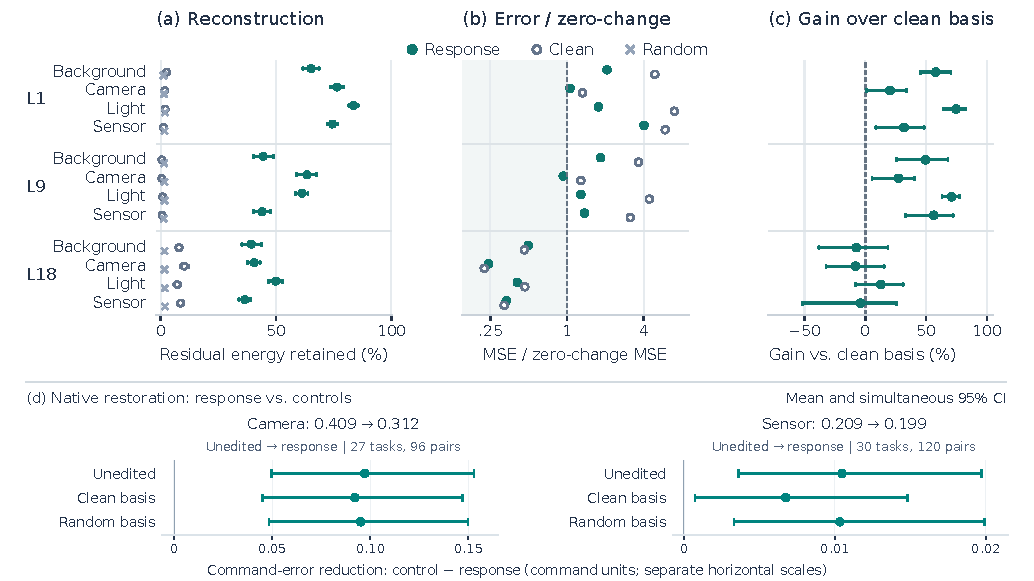
\includegraphics[width=\textwidth]{figure_readability_revision/frozen_figure3.pdf}
\captionof{figure}{\textbf{Shared directions retain unseen responses, and restoring them at L9 reduces command error.} (a--c) The same 404 LIBERO-Plus pairs on 28 tasks; each fit leaves out the test tasks and family. (a) Share of the centered response energy at the first generation step retained by 16 shared directions. (b) Readout error relative to predicting no change; below 1 beats no change (log axis). (c) Gain over clean-feature directions in predicting commands: positive favors the shared directions; panel (b) gives the no-change reference. (a,c) Pointwise 95\% task intervals. (d) Restoration at L9, a separate study: 96 Camera and 120 Sensor Noise cases on 27/30 tasks. Command error is the distance between the first five commands and those of the clean run. Points show error reductions (other run minus restoration); intervals are simultaneous 95\% over six comparisons. Headers give unedited $\rightarrow$ restoration error. Separate horizontal scales show the smaller Sensor Noise effect. All controls: Sec.~\ref{sec:allstep-restoration}.}
\label{fig:supp-complete-geometry}
\end{center}

\clearpage
\begin{center}
\centering
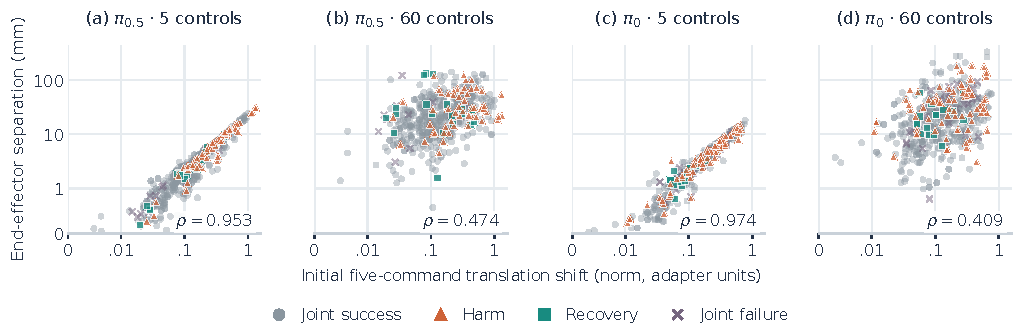
\includegraphics[width=\textwidth]{current_figures/figure6.pdf}
\captionof{figure}{\textbf{The change in the first five commands tracks motion closely after five controls and more weakly after 60.} Paired executions: both times use the same 516/536 pairs for $\pi_{0.5}$ and 526/536 for $\pi_0$, on all 40 tasks. A pair enters if its commands and its motion at both times passed validation, without the cross-family restriction of Fig.~\ref{M-fig:behavior}. Color gives the observed paired outcome; all outcome classes are included. $\rho$: task-weighted rank correlation across the plotted pairs. Shared symmetric-log axes are linear below 0.01 command units and 1\,mm. Pointwise 95\% intervals and paired early-minus-late differences: Sec.~\ref{sec:early-late-association}.}
\label{fig:supp-early-late}
\end{center}


\clearpage
\begin{center}
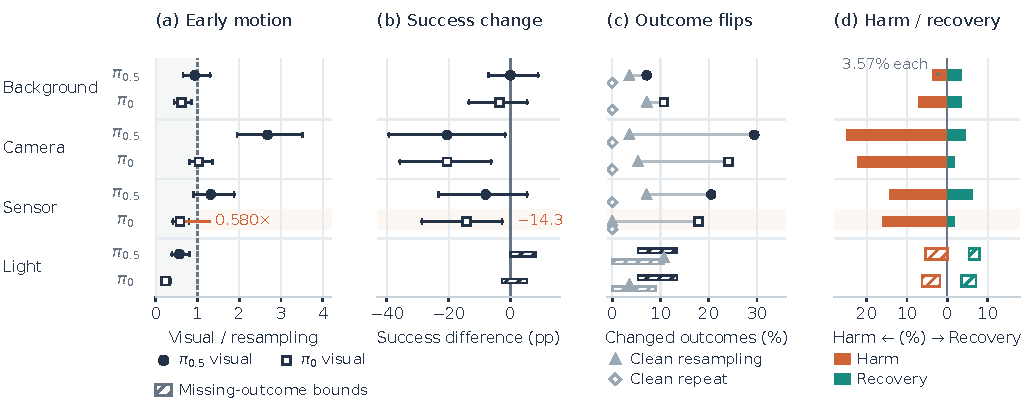
\includegraphics[width=\textwidth]{figure_readability_revision/frozen_figure7.pdf}
\captionof{figure}{\textbf{Motion, net success and paired outcomes show different effects of a perturbation.} 202 settings with a LIBERO-Plus difficulty level, 28 tasks per policy. (a) Motion ratio: end-effector separation after five controls relative to the separation between two clean runs with different policy noise (clean rerun). Ratios divide task-equal means, with pointwise 95\% task intervals; shading marks values below the clean rerun. Light has 43/48 settings on 26 tasks ($\pi_{0.5}$), 44/48 on 27 ($\pi_0$). (b) Success change with four-family-adjusted 98.75\% intervals. (c) Lines connect the rates of changed outcomes under the perturbation and under a clean rerun (descriptive). (d) Lost successes extend left and gained successes right; lengths are positive percentages. Hatching marks bounds over missing outcomes, distinct from sampling intervals. The highlighted row is $\pi_0$ Sensor Noise. Secs.~\ref{sec:supp-matched-motion} and~\ref{sec:five-arm}.}
\label{fig:supp-complete-outcomes}
\end{center}
